\chapter{Implementierung}
Die aufgestellten Anforderungen und das darauf basierende Design-Konzept kann nun in eine eigene Anwendung implementiert werden.
Dabei wird zuerst auf die Entwicklung auf iOS-Geräten eingegangen und anschließend die Technische Umsetzung dokumentiert.
Bei der Umsetzung wird auf die \Gls{i18n} geachtet, sodass es im Anschluss möglich ist die Anwendung mittels \Gls{l10n} in verschiedene Sprachen zu übersetzen.\pbreak%
%
Die Nutzung der Anwendung findet idealerweise auf einem Tablet statt, da dort mehr Platz für das Zeichnen und das Vornehmen von Einstellungen bereitsteht.
Für die Entwicklung wird die Entwicklungsumgebung \textit{Xcode} verwendet, welche Gerätesimulatoren für alle zur Verfügung stehenden iOS-Geräte bereitstellt.

\section{Entwicklung auf iOS-Geräten}
Wenn man einen nativen Ansatz verfolgt, um eine Anwendung auf iOS-Geräten zu entwickeln, stehen einem drei verschiedene Technologien zur Verfügung:
\textit{Objective-C}, \textit{Swift} und \textit{SwiftUI}.

\subsection{Objective-C und Swift}
Objective-C war lange Zeit die einzige Programmiersprache für Geräte von Apple, bis Swift im Jahre 2014 angekündigt wurde.
Des Weiteren ist Swift Open-Source und verfolgt den Ansatz plattformübergreifend genutzt werden zu können \parencite{APP2020}.
Im Vergleich zu Objective-C hat Swift eine modernere Syntax und weniger Verbosität im Programmcode.
Es wird nicht mehr in Header- und Implementierungs-Dateien unterschieden und der gesamte Aufbau erinnert an eine Kombination verschiedenster moderner Programmiersprachen.
Dies lässt sich leicht erklären, da Chris \textcite{LAT} – Hauptentwickler der Programmiersprache Swift – auf seiner Website sagte \blockquote{Of course, it also greatly benefited from the experiences hard-won by many other languages in the field, drawing ideas from Objective-C, Rust, Haskell, Ruby, Python, C\#, CLU, and far too many others to list}.
Im folgenden Listing \ref{lst:objc} wird eine Beispielimplementierung der Klasse \texttt{Vehicle} gezeigt, die eine Methode zum Öffnen eines Fensters besitzt.
Als Parameter können mit \texttt{percentage} der Prozentwert der Öffnung angegeben werden und mit \texttt{seat} übergeben werden, welches Fenster geöffnet werden soll.
Im Anschluss wird ein Objekt der Klasse erstellt und die Methode aufgerufen.
\codelisting{Implementierung der Vehicle-Klasse in Objective-C}{lst:objc}{objc-example.m}{objc}\\
Im Listing \ref{lst:swift} mit der Swift-Implementierung entfällt das Einbinden von Header-Dateien.%
%
Außerdem sind Methodenaufrufe und Initialisierungen von Objekten um einiges klarer und leserlicher, da im Vergleich zu Objective-C die umschachtelnden \texttt{[]} entfallen.
\codelisting{Implementierung der Vehicle-Klasse in Swift}{lst:swift}{swift-example.swift}{swift}

\subsection{SwiftUI}
Seit 2019 gibt es auch die Möglichkeit mittels \textit{SwiftUI} mobile Anwendungen für Apple Geräte zu entwickeln.
SwiftUI ist dabei weniger eine eigene Sprache, sondern eher ein deklarativer Ansatz in Swift User Interfaces zu bauen.
In normalen Swift Anwendungen wird für die Benutzeroberfläche das Framework \textit{UIKit} verwendet.
SwiftUI soll in Zukunft UIKit ablösen, sodass alle Anwendungen in Zukunft mittels SwiftUI entwicklet werden können.\pbreak%
%
Da SwiftUI noch relativ jung ist und regelmäßig neue Funktionen implementiert ist es für eine komplexere Anwendung ungeeignet.
Einfache Notizen- oder Todo-Apps lassen sich schnell und einfach bauen, doch für das Zeichnen auf Kartendaten müsste wieder auf Swift mit UIKit zurückgegriffen werden.

\subsection{Application Life Cycle}
\subsection{Entwurfsmuster}
Es gibt viele verschiedene Möglichkeiten die Architektur einer Software aufzubauen.
Bei einfachen iOS-Anwendungen wird dafür das Entwurfsmuster \ac{mvc} verwendet.
Obwohl es möglich ist für die eigene Anwendung ein anderes Entwurfsmuster zu verwenden, lohnt es sich das bereitgestellte zu nutzen, da das \Gls{sdk} viele Werkzeuge mitbringt, die automatisiert Dateien erstellen und verwalten können, solange man sich an das \ac{mvc}-Entwurfsmuster hält.
\subsubsection{Model-View-Controller}
Das \ac{mvc}-Entwurfsmuster teilt den Programmcode in die drei Bereiche \textit{Model}, \textit{View} und \textit{Controller} ein.
Jeder dieser Bereiche hat eine eigene Zuständigkeit und sollte bis auf die Kommunikation streng von den anderen getrennt sein.
\begin{figure}[h!]
	\centering
	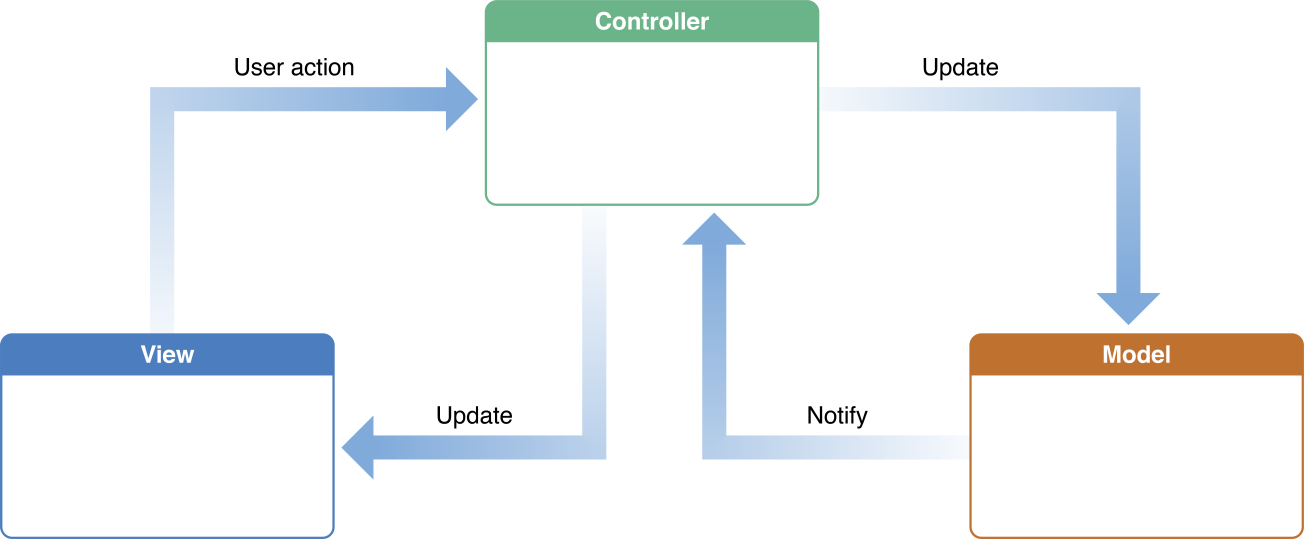
\includegraphics[scale=0.2]{images/model-view-controller}
	\caption{Darstellung der Model-View-Controller Beziehungen}
	\label{fig:model-view-controller}
\end{figure}
Die \textbf{Model}-Ebene beinhaltet den Code für das Datenmodell der Anwendung.\pbreak
Die \textbf{View} ist der Bereich, mit dem der Benutzer interagiert.
Programmcode auf der View-Ebene sollte keine Business-Logik enthalten, sondern nur Code, welcher die View aktualisiert.\pbreak
Die Aufgabe der \textbf{Controller} ist es die Model und Views zu verbinden.

\subsubsection{Delegation-Pattern}
Das Delegation-Pattern...

\subsection{Die Information Property List}
In jedem iOS-Projekt muss eine sogenannte \textit{Information Property List} vorhanden sein.
Diese kann als \texttt{Info.plist}-Datei an einer beliebigen Stelle im Projekt abgelegt sein, es muss nur der Pfad zu ihr hinterlegt werden.
Die Property List ist ein Key-Value-Store und basiert auf XML (siehe Listing \ref{lst:plist}).
In dieser Liste werden unter anderem der Name der Anwendung, die Version, die Buildnummer und weitere Einstellungen vorgenommen.
Außerdem werden in der Property List auch die Begründungstexte für Berechtigungsanfragen abgelegt.
Wenn eine Anwendung versucht den Zugriff auf das Mikrofon anzufragen, allerdings kein Begründungstext hinterlegt wurde, der dem Benutzer angezeigt werden kann, wird die Berechtigung nicht angefragt.
\codelisting{Beispielinhalt einer Property List}{lst:plist}{plist-example.plist}{xml}\\

\section{Technische Umsetzung}
\subsection{Autolayout}
\subsection{JSON Encoding und Decoding}
\subsection{Generics}
\subsection{Gesture Recognizers}
\subsection{MapKit Overlays}

\section{Lokalisierung der Anwendung}
\subsection{Localizable-Dictionary}
\subsection{ISO Country Codes}
